%! Suppress = MissingImport
\chapter{Proposed Solution to problem}\label{ch:proposed-solution-to-problem}
In chapter~\ref{ch:project-problem}, the program case was outlined describing the general idea and reasoning for the
project. This chapter builds upon that giving a mathematical description of the problem (\ref{sec:optimisation-problem}),
which allows the problem to be separated into two sub-problems: task auctioning (sections~\ref{sec:task-auctioning})
and resource allocation (\ref{sec:resource-allocation-solution}) that are each discussed with solution proposed.

\section{Optimisation problem}\label{sec:optimisation-problem}
%% Todo not sure how to start this section
%% The information that I wish to transfer is:

%% Todo add this section somewhere
The principle of flexibility for resource allocation, that is described in chapter~\ref{ch:project-problem}, is that
for certain resources, the time taken for an operation to occur, e.g.\ loading of a program, computing the program and
sending of results, etc, is proportional to the amount of resources allocated to completed the operation.
\footnote{This principle is not always true, for example, video decompression is a generally a single
thread operation thus this assumption doesnt work. However for this project we only consider operations that can be
parallelised effectively.}
Using this principle, a modified version of a standard resource allocation formulation can be described.

%% Todo original text
A sketch of the system is shown in Fig.~\ref{fig:system_model}.
We assume that in the system there is a set of $I = \{1,2,\ldots,\left|I\right|\}$ servers are heterogeneous in all
characters. Each server has a fixed availability of resources: storage for the code/data needed to run a task
(e.g., measured in GB), computation capacity in terms of CPU cycles per time interval (e.g., measured in FLOP/s),
and communication bandwidth to receive the data and to send back the results of the task after execution (e.g., measured in Mbit/s).
We denote these resources for server $i$: the storage capacity as $S_i$, computation capacity as $W_i$, and the communication capacity as $R_i$.

\begin{figure}
    \centering
    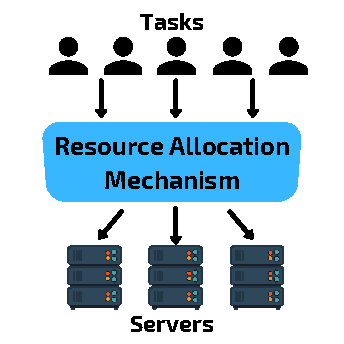
\includegraphics{figures/system_model.pdf}
    \caption{System model}
    \label{fig:system_model}
\end{figure}

There is a set $J = \{1,2,\ldots,\left| J \right|\}$ of  different tasks that require service from one of the servers
in set $I = \{1,2,\ldots, \left| I \right|\}$. To run any of these tasks on a server requires storing the appropriate
code/data on the same server. These could be, for example, a set of images, videos or CNN layers in identification
tasks. The storage size of task $j$ is denoted as $s_j$ with the rate at which the program is transferred to the server
$i$ at time $t$ being $s^{'}_{i,j,t}$. For a task to be computed successfully, it must fetch and execute instructions
on a CPU. We consider the total number of CPU cycles required for the program to be $w_j$, where the rate at which the
CPU cycles are assigned to the task on server $i$ at time $t$ is $w^{'}_{i,j,t}$. Finally, after the task is run and
the results obtained, the latter need to be sent back to the user. The size of the results for task $j$ is denoted with
$r_j$, and the rate at which they are sent back to the user is $r^{'}_{i,j,t}$ on server $i$ at time $t$. Every task
has a beginning time, denoted by $b_j$ and a deadline, denoted by $d_j$. This is the maximum time for the task to be
completed in order for the user to derive its value. This time includes: the time required to send the data/code to the
server, run it on the server, and get back the results. Therefore for the task to be successfully completed, it must
completed fulfill the constraint in equation~\eqref{eq:deadline}. These operations must occur in order (loading,
computing then sending of results) as a server couldn't compute a task that was not fully loaded on the machine.

\begin{align}
    \frac{s_j}{\sum^{d_j}_{t=b_j} s^{'}_{i,j,t}} + \frac{w_j}{\sum^{d_j}_{t=b_j} w^{'}_{i,j,t}}  +
    \frac{r_j}{\sum^{d_j}_{t=b_j} r^{'}_{i,j,t}} \leq d_j && \forall{j \in J}  \label{eq:deadline}
\end{align}

As server have limited capacity, the total resource usages for all tasks running on a server must be capped.
The storage constraint (equation~\eqref{eq:server_storage_capacity}) is unique as the previous amount
loaded in kept till the end of a program on server. While the computation capacity
(equation~\eqref{eq:server_computation_capacity} is the sum of compute used by all of the tasks on a server $i$ at time $t$ and the
bandwidth capacity (equation~\eqref{eq:server_bandwidth_capacity}) is the sum of loading and sending usages by tasks.
\begin{align}
    \sum_{j \in J} \left(\sum^{d_j}_{t=b_j} s^{'}_{i,j,t} \right) \leq S_i, && \forall{i \in I} \label{eq:server_storage_capacity} \\
    \sum_{j \in J} w^{'}_{i,j,t} \leq W_i, && \forall{i \in I, t \in T} \label{eq:server_computation_capacity} \\
    \sum_{j \in J} s^{'}_{i,j,t} + r^{'}_{i,j,t} \leq R_i, && \forall{i \in I, t \in T} \label{eq:server_bandwidth_capacity} \\
\end{align}

\section{Task Auctioning solution}\label{sec:task-auctioning}
If an agent wish to run on task on the cloud, the task can be put forward with its requirements of required storage,
computation, results data and deadline. In order for fast and truthful, a reverse Vickrey auction~\citep{vickrey}
will be implemented  where servers all submit their bid for the task with the winner being the server with the lowest
price but actually only gains second lowest price. The Vickrey auction is incentive compatible meaning that the dominant
strategy for bidding on a task is to bid your truthful value for a task. This should help server as they dont need
to learn how to outbid another agent as it only needs to consider its own evaluation.
As there is also only a single round of bidding compared to alternative auctions like English or Dutch
auctions, this makes auctioning fast no matter the number of servers and it also allows for a reserve price to be used.

In order to calculate the price of the task for a server requires a understanding the resource requirements of the task,
the future supply and demand for tasks and the resource requirements of currently allocated tasks. Due to the complexity
in creating a heuristic that can accurately use this information and the amount of memory required for a table based
approach. Because of this, a long/short term memory (LSTM) will be implemented~\citep{LSTM}  for evaluating the price
of a task. The justified for the use of this network over other neural network models is explained in
Section~\ref{sec:justification-for-task-auctioning}. The network would take as input, the currently
allocated tasks requirements, the possible task requirements and the server resource capacity, outputting just a single
value representing the price of the task, normalised between 0 and 100.

\section{Resource allocation solution}\label{sec:resource-allocation-solution}
In previous work~\citep{FlexibleResourceAllocation}, that utilised a single shot problem case where jobs wouldnt arrive
over time, the resource speeds set were fixed and assumed that a task loading, computing and sending result
occurred concurrently. With the addition of time, results in these assumptions not to hold anymore as tasks contain
stages for the loading, computing and sending of results thus requiring allocated resource speeds to change over time.
Therefore at each time step, a server needs to reallocate all of its resource to its currently allocated tasks as
some tasks will have completely one of its stages.

In order to select how to allocate resource to tasks, this problem doesn't seem as complex as the pricing in
section~\ref{sec:task-auctioning} therefore simple heuristic and long/short term memory neural network will be
implemented and compared. This is justified in section~\ref{sec:justification-for-task-auctioning}. The LSTM will take as input, all of
the currently allocated tasks that are at a particular stages resource requirements and the task's resource requirement
returning a single value between 1 to 100. Once this is completed for each job, the percentage of the total values will
be assigned to each task.

\section{Environment problem}\label{sec:markov-decision-process-description}
%% Todo write about MDP
